\documentclass[11pt]{article}
\usepackage{graphicx}
\usepackage{amssymb}
%\usepackage[nomarkers]{endfloat}
\usepackage{natbib}
\usepackage{setspace}
\usepackage{wasysym}
\usepackage{wrapfig}

\textwidth = 7 in
\textheight = 9 in
\oddsidemargin = -0.5 in
\evensidemargin = -0.5 in
\topmargin = 0.0 in
\headheight = 0.0 in
\headsep = 0.0 in
\parskip = 0.1in
\parindent = 0in
\renewcommand{\Pr}{\mathbb{P}}
\usepackage{paralist}
\usepackage{url}
\newcommand{\href}[2]{\url{#2}}
\usepackage{hyperref}
\hypersetup{backref,   linkcolor=blue, citecolor=red, colorlinks=true, hyperindex=true}
\begin{document}
notes from the week of Feb.~25, 2019 \\
\tableofcontents


\section{Revisiting the time to MRCA from mutation counts}
\subsection{the data}
Now we'll add my sequence to the previous example.
We have a tree with 1 or 2 MRCAs.
Our data is
$X=[3,2,6]$,
so our sample size is $n=3$.

\section{the likelihood}\label{M1model}
Given that we have worked on similar problems recently, we probably would reach
for the Poisson likelihood:
\begin{eqnarray}
\Pr(X\mid ut_1, ut_2, ut_3)& = & \prod_{i=1}^{n} \Pr(x_i\mid ut_i)\\
& = & \prod_{i=1}^{n} \frac{(ut_i)^{x_i}e^{-ut_i}}{x_i ! }
\end{eqnarray}
This is not wrong, but it fails to accurately convey the constraints on the parameter.
If you and JKK share a mitochondrial MRCA more recently than either of you do with me, then $t_1=t_2$ and $t_3> t_1$.

We can express those constraints on the parameters mathematically as an expression of the domain.
In this case: 
\begin{eqnarray}
    t_1, t_2, t_3, u & \in &  \mathbb{R}\\
    0 & < u < & \infty\\
    0 & < t_1 < & \infty\\
    t_1 & = & t_2 \\
    t_1 & \leq & t_3
\end{eqnarray}
where the first line says that all four parameters are real numbers (not integers, 
not complex numbers, {\em etc.}), and then the equations and inequalities constrain
the feasible range of them.

This is fine and it works fine.

Sometimes it is easier to reparameterize in a way that makes the parameters more
``orthogonal'' (in some vague sense).
What occurs to me is to use $\omega$ to represent a mutation-rate-scaled waiting
time to the previous coalescence event.
That occurs to me because it is the kind of thing we often do in coalescent theory.
It may not occur to you, and that is OK -- you can get the right answers without
this reparameterization.

Specifically:
\begin{eqnarray}
    \omega_1, \omega_2 & \in &  \mathbb{R}\\
    0 & < \omega_1, \omega_2 < & \infty\\
     ut_1 = ut_2 & = & 2\omega_1  \\
    ut_3 &= & 2\omega_2 + \omega_1
\end{eqnarray}

We'll call this model $M_1$ (3 more coming later).
\begin{eqnarray}
\Pr(X\mid \omega_1,\omega_2, M_1)& = & \prod_{i=1}^{n} \Pr(x_i\mid \omega_1,\omega_2)\\
& = &
 \frac{\omega_1^2e^{-\omega_1}\omega_1^3e^{-\omega_1}\left(\omega_1+2\omega_2\right)^6e^{-(\omega_1+2\omega_2)}}{2!3!6!} \\
& = & \frac{1}{2!3!6!}\left[\omega_1^5e^{-2\omega_1}\right]
\left[\left(\omega_1+2\omega_2\right)^6e^{-(\omega_1+2\omega_2)}\right] \\
\ln L(\omega_1,\omega_2, M_1) & = & -\ln(2!3!6!)+ \left[5 \ln(\omega_1) -2\omega_1\right] +
\left[6\ln\left(\omega_1+2\omega_2\right) -\omega_1- 2\omega_2)\right] \\
& = & -\ln(2!3!6!)+ 5 \ln(\omega_1) -3\omega_1 +
6\ln\left(\omega_1+2\omega_2\right) - 2\omega_2
\end{eqnarray}
where the [] braces just help us see that the likelihood is coming from 2 paths in the tree: the one between JKK and you $x_1+x_2 = 5$ and the one that says that MTH
is 6 mutations away from that common ancestor $x_3 = 6$

You can derive how $\hat{\omega_1}=2.5$ based soley on $x_1+x_2 = 5$.
However it is not clear if that is actually the maximum likelihood
if we use all the data (and we should always use all of the data).

In this parameterization $\omega_2$ does not affect the probability of $x_1, x_2$ at 
all. 
But $\omega_2$ and $\omega_1$ both appear in the log likelihood from $x_3$.
So if the MLE of $\omega_1$ from $x_3$ does not agree with 2.5, then we 
    will have some tension in the information provided by $x_1, x_2$
    and $x_3$ about what $\omega_1$ should be and the estimate will be 
    some compromise.

We can figure out MLE by taking the {\em partial} derivatives with
    respect to each of the parameters and then
    finding the values of the parameters that make
    both partial derivatives 0 (while also paying attention to
    the boundaries as possible maxima):

\begin{eqnarray}
\frac{\partial\ln L}{\partial \omega_1} & = &
    \frac{5}{\omega_1} -3  + \frac{6}{\omega_1+2\omega_2} \\
\frac{5}{\hat{\omega}_1}  + \frac{6}{\hat{\omega}_1+2\omega_2} & = & 3 \\
\frac{\partial\ln L}{\partial \omega_2} & = &
    \frac{(6)(2)}{\omega_1+2\omega_2} - 2 \\
    6 & = & \omega_1+2\hat{\omega}_2 \\
    3 - \frac{\omega_1}{2} & = & \hat{\omega}_2 
\end{eqnarray}
If (for the time being) we ignore the possibility 
of one of the parameters being at the edge of its feasible range, then
    we can use our solutions for $\hat{\omega}_1$ and
    $\hat{\omega}_2 = 3 - \frac{\omega_1}{2}$ at the same time:
\begin{eqnarray}
\frac{5}{\hat{\omega}_1}  + \frac{6}{\hat{\omega}_1+2\hat{\omega}_2} & = & 3 \\
\frac{5}{\hat{\omega}_1}  + \frac{6}{\hat{\omega}_1+6 - \hat{\omega}_1} & = & 3 \\
\frac{5}{\hat{\omega}_1}  + \frac{6}{6} & = & 3 \\
\frac{5}{\hat{\omega}_1}  & = & 2 \\
\hat{\omega}_1 & = & 2.5 \\
\hat{\omega}_2 & = & 3 - \frac{2.5}{2} = 1.75 
\end{eqnarray}
Once again these MLE make sense because you predict 5 difference between your sequence and JKK, and
 $\hat{\omega}_1 + 2\hat{\omega}_2 = 6$, which is exactly the number of changes along the branch
leading to my sequence.

Figure \ref{fullLnLOut6} shows the
log-likelihood broken down into the effects of $x_1+x_2=5$ and $x_3=6$,
 and the full log-likelihood.
Note that the $\ln L$ in the right panel is simply the sum of 
    the $\ln L$ components in the previous panels.

\begin{figure}[h]
\hskip-0cm \includegraphics[scale=.33]{images/lnL-from-x1.png}
\hskip-1cm \includegraphics[scale=.33]{images/out-6-root-spanning-lnL-contour.pdf}
\hskip-1cm \includegraphics[scale=.33]{images/out-6-full-lnL-contour.pdf}
\caption{(LEFT) $\ln\Pr(X=5\mid\omega_1)$ -- this is partial log-likelihood obtained from the fact that there are 5 changes across $\nu$ (or $\omega_1$).
(CENTER) contour plot of $\ln\Pr(X=6\mid\omega_1, \omega_2)$ -- this is partial log-likelihood obtained from the fact that there are 6 changes across the branch that spans the root of the tree.
(RIGHT) $\ln\Pr(X=[5,6]\mid\omega_1, \omega_2)$ with a dot on the MLE and contours every 0.5 log-liklihood unit intervals}\label{fullLnLOut6}
\end{figure}

\section{A second model}\label{M2model}
If we consider the possibility that you and I share a MRCA of
    our mitochondria more recently than either of us do with JKK,
    then we can formulate a very similar model.
We can call it $M_2$.
Now $\omega_{1,2}$ denotes the branch length from the present to the MRCA of you and MTH.
$\omega_{2,2}$ will denote the branch length from that ancestor
    to our common ancestor with JKK.
Here the second 2 in the subscript is just helping us not confuse
    the omegas between the models.

Our data doesn't change of course.
On the shorter path we have 2 and 6 changes.
The 3 difference between JKK and the MRCA of us is now the
    stretched out over the 2 branches that span the root of the
    tree.

Figure \ref{modelNomen} sketches out the 4 models we'll consider.

\begin{figure}[h]
\hskip-0cm 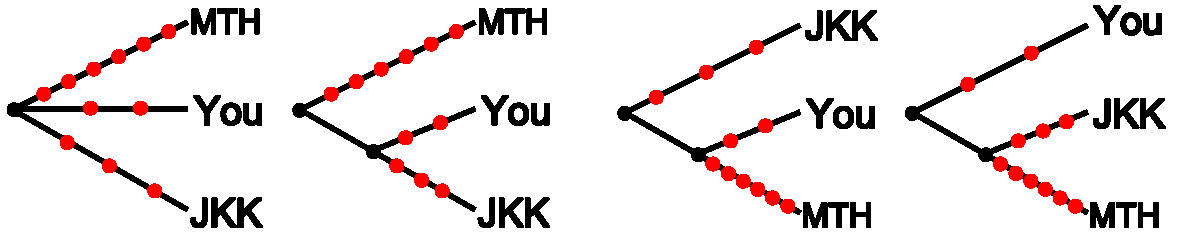
\includegraphics[scale=.75]{images/model-figures.pdf}\par
\hskip 5em $M_0$
\hskip 9em $M_1$
\hskip 9em $M_2$
\hskip 9em $M_3$

\caption{Nomenclature of models. $M_1$ is described in section 
\ref{M1model}, and $M_2$ is described in section \ref{M2model}}
\label{modelNomen}
\end{figure}  


The likelihood still connects the model to the data by assuming that 
    the data are Poisson-distributed counts with an expectation
    equal to the sum of branch lengths covered.
Skipping some of the algebra we get:

\begin{eqnarray}
\Pr(X\mid \omega_{1,2},\omega_{2,2}, M_2)& = &
 \frac{1}{2!3!6!}\left[\omega_{1,2}^8e^{-2\omega_{1,2}}\right]
\left[\left(\omega_{1,2}+2\omega_{2,2}\right)^3e^{-(\omega_{1,2}+2\omega_{2,2})}\right] \\
\ln L(\omega_{1,2},\omega_{2,2}, M_2) & = &
-\ln(2!3!6!)+ 8 \ln(\omega_{1,2}) -3\omega_{1,2} +
3\ln\left(\omega_{1,2}+2\omega_{2,2}\right) - 2\omega_{2,2}\\
\frac{\partial\ln L}{\partial\omega_{1,2}} & = & 
\frac{8}{\omega_{1,2}} -3 + \frac{3}{\omega_{1,2} + 2\omega_{2,2}} \label{partialOne}\\
\frac{\partial\ln L}{\partial\omega_{2,2}} & = & 
\frac{6}{\omega_{1,2} + 2\omega_{2,2}} -2 \\
\hat{\omega}_{2,2} & = & 1.5 - \frac{\omega_{1,2}}{2} \label{twoFromOne}\\
\frac{8}{\hat{\omega}_{1,2}} -3 + \frac{3}{\hat{\omega}_{1,2} + 3 - \hat{\omega}_{1,2}} & = & 0 \\
\frac{8}{\hat{\omega}_{1,2}} -2 & = & 0 \\
\hat{\omega}_{1,2} &= & 4
\end{eqnarray}
This is a pleasing solution when you look at the fact that 
we have a total of 8 changes over the 2 branches of length $\omega_{1,2}$.
It is less pleasing when you plug into equation (\ref{twoFromOne})
and find that $\hat{\omega}_{2,2} = -0.5$.
While that does maximize the likelihood (and in fact gives us the
same likelihood as we found in model $M_1$), this
combination of parameters also violates the feasible range of parameter $\omega_{2,2}$ which cannot be negative.

Looking at the likelihood surface (see Figure \ref{fullLnLOut3}) makes it clearer what is going on.
Once you prefer a value of $\omega_{1,1}$ that is greater
    than the number of changes that span the root of the tree,
    then you prefer smaller and smaller values of $\omega_{2,2}$

In this case we can find the MLE of $\omega_{1,2}$ conditional
    on $\omega_{2,2} = 0$ by simply substituting this
 into the equations from the partial derivative (equation
 \ref{partialOne}):
\begin{eqnarray}
\frac{\partial\ln L}{\partial\omega_{1,2}} & = & 
\frac{8}{\omega_{1,2}} -3 + \frac{3}{\omega_{1,2} + 2\omega_{2,2}} \\
\frac{8}{\hat{\omega}_{1,2}} -3 + \frac{3}{\hat{\omega}_{1,2}} & = & 0\\
\frac{11}{\hat{\omega}_{1,2}} & = & 3\\
\hat{\omega}_{1,2}&  = & \frac{11}{3}
\end{eqnarray}

This answer also makes sense because if the branch to the earliest common ancestor has length 0, then
 you have 3 equally distant (in terms of time) tips with 
 a total of 11 changes.
Under the molecular clock the best branch length is one that
    implies 11/3 changes per branch.

This is also the likelihood under model $M_0$. 
As an exercise, you should also be able to verify that this
is the best likelihood that you can get under $M_3$.

\begin{figure}[h]
\hskip-1cm \includegraphics[scale=.5]{images/out-3-root-spanning-lnL-contour.pdf}
\hskip-1cm \includegraphics[scale=.5]{images/out-3-full-lnL-contour.pdf}
\caption{(LEFT) Contour plot of $\ln\Pr(X=3\mid\omega_{1,2}, 
\omega_{2,2})$ -- this is partial log-likelihood obtained from the fact that there are 3 changes across the branch that spans the root of the tree.
(RIGHT) $\ln\Pr(X=[8,3]\mid\omega_{1,2}, \omega_{2,2})$ with a dot on the MLE and contours every 0.5 log-liklihood unit intervals}\label{fullLnLOut3}
\end{figure}



\end{document}

